\documentclass[12pt,letterpaper]{report}

\usepackage[utf8]{inputenc}
\usepackage[spanish]{babel}
\usepackage{graphicx}
\usepackage{float}
\usepackage{array}
\usepackage[left=3cm,right=3cm,top=2cm,bottom=2cm]{geometry}
\usepackage[breaklinks,colorlinks=true,linkcolor=black,citecolor=blue,urlcolor=black]{hyperref}

\makeindex

\title{Tesis}

\renewcommand{\baselinestretch}{1.2}
\begin{document}
	\pagenumbering{roman}	
	\renewcommand{\listtablename}{Índice de tablas}
	\renewcommand{\tablename}{Tabla}
	\renewcommand{\bibname}{Referencias bibliográficas}	
%	esto es para que las listas anidadas salgan con numeros
	\renewcommand{\labelenumii}{\arabic{enumi}.\arabic{enumii}}
	\renewcommand{\labelenumiii}{\arabic{enumi}.\arabic{enumii}.\arabic{enumiii}}
	\renewcommand{\labelenumiv}{\arabic{enumi}.\arabic{enumii}.\arabic{enumiii}.\arabic{enumiv}}
	
	
	\pagestyle{empty}		
	\thispagestyle{empty} 
	
 	\begin{titlepage}

\centering

{
\includegraphics[width=0.5\textwidth]{imagen/cujae}\par}

\vspace{3.5cm}

{\scshape\LARGE Sistema para el entrenamiento de operarios en la Industria Alimentaria \par}
%%{\scshape\Large SISTEMA PARA EL ENTRENAMIENTO DE OPERARIOS EN LA INDUSTRIA ALIMENTARIA \par}
\vspace{1cm}

{\bfseries\Large Trabajo de Diploma para Optar por el Título de Ingeniería en Informática\par}
\vspace{3.5cm}

{\bfseries\Large Autor:} { \Large Mónica Montoto Montané \par}
{\bfseries\Large Tutor: }{\Large Dra. Raisa Socorro Llanes \par}
\vfill

{\Large La Habana, Cuba \par}

\large{\mifecha\today}

\end{titlepage}



	%\include{dec_autoria}
	%\include{opinion_tutor}
	%\chapter*{Dedicatoria}
A mis padres, por siempre estar a mi lado, por la confianza depositada, por los empujones cuando no quería seguir, por motivarme, por hacerme una persona de bien y cada día luchar por mi futuro; a ellos, se los debo todo. Una vez me dijeron que la idea de criar hijos no es para que te acompañen cuando tú estés viejo, es para asumir la responsabilidad de criar humanos funcionales, comprometidos con la naturaleza y la sociedad. Este título también es de ustedes, porque lo sufrieron tanto como yo, y se los entrego con la promesa de que seguiré intentando ser una persona de bien, y que se sientan tan orgullosos como yo estoy de ustedes.

A mi tutora Raisa, que aceptó el reto de cuidarme y apoyarme, y lo hizo de la mejor manera. Sin dudas puedo decir, que tuve la suerte de conocer a una de las mejores profesionales que trabajan en la universidad. Gracias por enseñarme, por apoyarme y tenerme paciencia. A usted no solo la quiero, yo la admiro.
	%\chapter*{Agradecimientos}
Quiero dedicar el siguiente trabajo a todas aquellas personas que lucharon porque se hiciera realidad, y no hablo solo de la tesis, si no de todos aquellos compañeros que tuve apoyándome desde un inicio para que hoy pudiera estar aquí.
	
	\section*{Resumen}
La Industria Alimentaria en Cuba juega un rol muy importante dentro de la economía del país. Cuando existe una falla en su proceso productivo, no siempre están presentes los expertos para su posible solución, ya que no todos los técnicos están preparados para tomar decisiones correctas en determinadas circunstancias. En ese caso, se detiene la producción hasta que aparezca el trabajador que pueda resolver la falla ocurrida, provocando pérdidas en numerosas áreas y sectores. Es por ello que, esta industria, presenta la necesidad de capacitar a todos sus operarios ante los procesos que en ella se desarrollan.

Para brindarle una solución a esta problemática se desarrollaron, por el Instituto de Investigaciones de la Industria Alimentaria (IIIA) y la Facultad de Ingeniería Informática e Ingeniería Química de la CUJAE, un Sistema Experto para el Control de Procesos Químicos (SECPROIT) y un Generador de Bases de Conocimientos.

Este sistema experto SECPROIT, tiene como objetivo evaluar las decisiones que toman los operarios ante diferentes situaciones críticas y brinda a los jefe los resultados de las mismas y cómo se van superando sus trabajadores ante cada proceso. Actualmente, dicho sistema, presenta ciertas limitaciones que impiden su correcto funcionamiento, por lo que es necesario realizar una actualización del mismo.

Una vez logrado este objetivo se podrán resolver los problemas de la Industria Alimentaria, planteados al inicio de este resumen. A esta investigación se le atribuye un valor práctico, ya que este sistema (artefacto de salida) será implementado en las Industrias Azucareras Cubanas.

\vfill

\begin{description}
	\item[Palabras claves:]{Industria Alimentaria, proceso productivo, operario, Instituto de Investigaciones de la Industria Alimentaria (IIIA), situación crítica, Sistema Experto para el Control de Procesos Químicos (SECPROIT), Generador de Bases de Conocimientos, sistema experto, artefacto de salida.}
\end{description}



	\section*{Abstract}
The Food Industry in Cuba plays a very important role in the economy, so a problem in this sector should be avoided at all costs. It currently presents the need to train all its operators in the production processes that are developed, since it consists of many irregularities when working on them. When there is a fault, experts are not always present for its possible solution, since not all technicians are prepared to make the correct decisions in certain circumstances. In this case, the production process is stopped until an expert appears who can resolve the fault that has occurred, causing losses in many areas and thus affecting the economy.

As a result of this situation, the Food Industry Research Institute (IIIA), in conjunction with the Faculty of Computer Engineering and Chemical Engineering of CUJAE, in search of a solution, developed an Expert System for the Control of Chemical Processes ( SECPROIT) and a Knowledge Base Generator.

The SECPROIT expert system aims to evaluate the decisions made by operators in different critical situations and provides managers with their results and how their workers improve in each process. At this time, the system has certain limitations that prevent it from working properly, so it is necessary to update it. Once this objective has been achieved, the problems of the Food Industry, raised at the beginning of this summary, can be resolved.

\vfill

\begin{description}
	\item[Keywords:]{Food Industry, production process, operator, Food Industry Research Institute (IIIA), critical situation, Expert System for the Control of Chemical Processes (SECPROIT), Knowledge Base Generator, expert system.}
\end{description}
	
	\pagestyle{plain}	
	
	\tableofcontents	
	\pagebreak	
	
	\listoftables
	\pagebreak
	
	\listoffigures	
 	\clearpage 

	\pagenumbering{arabic}
	
	\phantomsection
	\addcontentsline{toc}{chapter}{Introducción}
	\pagestyle{fancy} 
	
	\chapter*{Introducción}
En la actualidad, el desarrollo tecnológico se ha convertido prácticamente en una obligación para la mayoría de los entornos laborales, industriales y sociales. En un mundo tan globalizado, que avanza y se supera con una rapidez vertiginosa, no resulta de extrañar que se exijan mejores condiciones y prestaciones. A partir de estas demandas, surge la necesidad de establecer nuevas técnicas en las grandes empresas que, de manera automática, faciliten todo tipo de actividades, desde lo laboral y comercial, hasta lo cotidiano \cite{avanceTecnologico}. 
Estas exigencias requieren nuevos desafíos, sin incluir los retos tecnológicos ya mencionados. Los avances técnicos traen consigo la necesidad de contar con factores humanos capacitados para responder ante este nuevo desarrollo científico \cite{invstCibernCuba}. 

Cuba no está ajena a esta nueva revolución tecnológica. El país está abocado a la creación y fortalecimiento de programas de posgrado que consoliden, complementen, profundicen y originen nuevos conocimientos, inmersos en áreas relacionadas con estos cambios de la era digital. De esta forma se proporcionan herramientas para afrontar retos, tomar decisiones y solucionar problemas de la sociedad cubana en general \cite{avanceTecnologico}.

El empleo de una tecnología de software propia reduce el tiempo de desarrollo y puesta marcha de la misma, minimiza el costo, aporta gran flexibilidad y eficiencia en las operaciones, mejora significativamente la trazabilidad de los procesos y facilita el trabajo a partir de diseños amigables de la interfaz hombre-máquina \cite{industriaCubana}.
Es por ello que, en Cuba, constantemente se trabaja en función de desarrollar nuevos sistemas que permitan un avance técnico significativo.
Por citar un ejemplo, la Industria Farmacéutica Cubana está compuesta por procesos tecnológicos de elevada complejidad, que necesitan cumplir con exigentes indicadores de calidad en la producción de medicamentos. A esta industria se le empleó una metodología que permitió automatizar la mayoría de sus procesos. Esta, ha significado un ahorro al país superior a tres millones y medio en moneda convertible en los últimos cinco años, un gran beneficio gracias al avance tecnológico \cite{industriaFarmceutica}.

En ocasiones, las ventajas competitivas que se obtienen con el uso de la tecnología, pueden verse afectadas por diversos riesgos, lo que provoca una posibilidad de pérdida hacia el futuro. Aunque son un hecho probabilístico sobre el que se tiene cierta incertidumbre, porque pueden ser provocados por factores internos o externos a la organización, tienen el poder de originar efectos indeseados en el cumplimiento de los objetivos de las instituciones. 
Ante esta realidad, ha surgido como necesidad la gestión de riesgos, con el propósito de lograr ejercicios de planeación y ejecución más acertados.
De esta situación no escapa la Industria Cubana y como parte de ella, la Industria Alimentaria \cite{CONVENCION2019}.

La Industria Alimentaria Cubana juega un rol muy importante dentro de la economía del país. Se caracteriza por trabajar de manera ininterrumpida, con un personal que cambia frecuentemente. Esta situación dificulta el entrenamiento de sus procesos productivos, ya que no cuenta con suficientes especialistas para la capacitación de los trabajadores. Al generarse una falla en un proceso, existe el inconveniente de una posible ausencia de expertos que encuentren una solución al problema, ya que todos los técnicos no tienen el mismo nivel de preparación para tomar decisiones ante fallas en determinadas circunstancias. En este caso, resulta entonces necesario paralizar el proceso productivo hasta localizar al experto que solucione el problema detectado, lo que genera pérdidas de recursos y un incumplimiento en el tiempo de producción \cite{gestorBases}.

El Instituto de Investigación de la Industria Alimentaria (IIIA) posee un capital humano especializado y de prestigio que a lo largo de los años, logró resultados científico-técnicos consistentes en la creación de aditivos, extensores alimenticios y la fortificación con vitaminas y minerales de alimentos seleccionados. El propósito de esta institución es lograr ventajas competitivas sostenibles en las industrias cubanas \cite{anaMailen}. 
Para darle solución al problema de la Industria Alimentaria, planteado anteriormente, este instituto, en conjunto con las facultades de Ingeniería Química e Ingeniería Informática (ambas de la CUJAE), desarrolló un Sistema Experto para el Control de Procesos Químicos (SECPROIT) y un Generador de Bases de Conocimiento.

El Generador de Bases de Conocimiento es el encargado de crear las bases de información para los diferentes procesos químicos que ocurren en una fábrica. Cada base contiene un grupo de variables, cada una con sus características y clasificaciones. De cada variable se conocen las causas que pueden provocar un estado de riesgo o alarma. De cada causa, se conocen las recomendaciones a seguir para minimizar los riesgos en el proceso productivo. A partir de estos datos, el generador elabora un conjunto de ficheros que luego serán utilizados por el SECPROIT \cite{anaMailen}.

El Sistema Experto para el Control de Procesos Químicos (SECPROIT) tiene como objetivo asesorar la toma de decisiones durante la ejecución de un proceso. A partir de los datos obtenidos por el Generador de Bases de Conocimiento, este sistema produce un conjunto de entrenamientos para los operarios de la fábrica. En cada prueba, el usuario debe escoger las variables que considere en estado de alarma, señalar sus posibles causas y seleccionar las recomendaciones a seguir. Cada prueba contiene tres etapas: variables, causas y recomendaciones. Estas evaluaciones son utilizadas para advertir los conocimientos de los trabajadores y la capacidad que posee cada uno \cite{elena}.

Actualmente el sistema SECPROIT posee ciertas limitaciones que impiden que sea implementado en las industrias:
\begin{itemize}
\item al generar o evaluar los entrenamientos, la información utilizada se extrae directamente de los ficheros obtenidos por el Generador de Bases de Conocimiento, lo que resulta una demora extra
\item solo existe un método de pregunta
\item el resultado del entrenamiento está dado por la cantidad de preguntas correctas que se respondieron, sin tener en cuenta el tiempo utilizado
\item en la última etapa, las recomendaciones, no se evalúan correctamente los resultados ni se muestra la puntuación obtenida
\item los entrenamientos se realizan de manera continua, sin posibilidad de pausa
\item las etapas aparecen de manera consecutiva, sin importar si la anterior fue aprobada o no, ya que los resultados solo influyen en la evaluación final (aparecen etapas innecesariamente)
\item los procesos se pueden evaluar una sola vez, es decir, por cada proceso existe un único entrenamiento, lo que limita la capacidad de aprendizaje del trabajador
\item los reportes del sistema no brindan toda la información requerida para conocer la capacidad del trabajador
\item las visuales del sistema son poco intuitivas, con colores oscuros y de diversos tamaños, lo que resulta poco amigable para el usuario
\end{itemize}

A partir de estas restricciones se intuyen un número de cambios necesarios a realizar. Estas modificaciones deben abarcar tanto la lógica programada, como su base de datos, sus interfaces de usuario y la estructura del sistema. Es decir, son requeridas diversas transformaciones en todas las capas internas del SECPROIT.
Es por ello que, una actualización desde el propio sistema, resulta más trabajosa que realizar un proyecto nuevo. Esto se debe a que modificar un código escrito, para adaptarlo a una nueva estructura y una nueva base de datos, resulta más complejo que elaborarlo de cero \cite{Plecka2013}.

Partiendo de este principio, resulta evidente que, la solución a esta situación problemática, es desarrollar un nuevo sistema tomando como origen el SECPROIT.
Esta actualización debe poder resolver el problema de investigación que se planteaba al principio: 
\textsl{¿Cómo lograr una completa capacitación de los operarios de la Industria Alimentaria, ante la toma de decisiones en una situación crítica?}

Por lo tanto, el objetivo general de esta investigación es: 
\begin{itemize}
\item Desarrollar un sistema capaz de adiestrar a los operarios de la Industria Alimentaria, tomando como guía el sistema SECPROIT, pero solucionando las limitaciones que este actualmente presenta.
\end{enumerate}

Para poder cumplir con el objetivo de esta investigación, deben completarse una serie de objetivos específicos, y cada uno, presenta un grupo de tareas a desarrollar:
\begin{enumerate}
\item Decidir con qué tecnologías se realizará el nuevo sistema
\begin{itemize}
\item Analizar los requisitos funcionales que debe cumplir el sistema
\item Seleccionar las tecnologías con las que se trabajará
\end{itemize}
\item Modelar la actualización del SECPROIT, tomando como base el sistema anterior
\begin{itemize}
\item Realizar diagramas auxiliares para comprender y estructurar el nuevo sistema (diagrama de caso de uso, modelo de dominio, diagrama de actividades, entre otros)
\end{itemize}
\item Implementar la nueva base de datos a partir del modelo resultante en el objetivo anterior
\begin{itemize}
\item Diseñar la nueva base de datos
\end{itemize}
\item Programar el sistema en cuestión, teniendo en cuenta las limitaciones presentes en la versión actual
\begin{itemize}
\item Implementar las funcionalidades que permitan la administración del sistema
\end{itemize}
\item Implementar las nuevas interfaces, rectificando lo señalado en el sistema anterior
\begin{itemize}
\item Realizar el diseño de las nuevas interfaces
\end{itemize}
\item Programar el entrenamiento de los operarios a partir de la información recibida por el Generador de Bases de Conocimiento
\begin{itemize}
\item Implementar la generación de preguntas asociadas a la evaluación del estado de las variables (fase de entrenamiento)
\item Implementar la generación de preguntas asociadas a la evaluación de las causas del estado de una variable (fase de entrenamiento)
\item Implementar la generación de preguntas asociadas a la evaluación de las recomendaciones del estado de una variable (fase de entrenamiento)
\item Implementar la configuración del proceso de evaluación asociado a un proceso en específico
\item Implementar la conexión con el JBOSS para obtener las respuestas correctas para las preguntas asociadas a las causas y recomendaciones
\item Implementar proceso de evaluación parcial para cada etapa
\item Implementar evaluación integral del operario en un proceso
\end{itemize}
\item Realizar pruebas al nuevo sistema resultante
\begin{itemize}
\item Diseño de las pruebas al sistema
\item Ejecución de las pruebas y experimentos al sistema
\end{itemize}
\item Desplegar la aplicación en la Facultad de Ingeniería Química, para luego implementarla en las industrias
\begin{itemize}
\item Crear un manual de usuario del nuevo sistema
\end{itemize}
\end{enumerate}

Esta investigación tiene como objeto de estudio: los sistemas de entrenamiento automatizados, los sistemas expertos y los sistemas de información basados en reglas de producción. De ellos, se centra la atención en el campo de acción que comprende el Sistema Experto para el Control de Procesos Químicos (SECPROIT).

Como artefacto de salida se obtiene la actualización de un sistema de entrenamiento (una aplicación práctica). Esta aplicación permitirá capacitar a los operarios de las industrias, específicamente a los de la Industria Alimentaria Cubana, por lo que se obtiene un valor práctico de gran importancia para la sociedad.	
	
	\renewcommand{\chaptermark}[1]{\markboth{\chaptername \, \thechapter. #1}{}}

	\chapter*{Capítulo 1 \vspace{0.5cm} \break Fundamentos teóricos}
\setcounter{chapter}{1}
\addcontentsline{toc}{chapter}{Capítulo 1: Fundamentos teóricos}

\section{Sistemas de capacitación laboral}
La capacitación laboral es un método aplicado por las empresas para que su personal adquiera nuevos conocimientos profesionales. Por lo general, se produce ante un ascenso o incorporación, aunque no son los únicos motivos. Busca perfeccionar al colaborador en su puesto laboral, en función de las necesidades de su empresa. Es un proceso estructurado con metas bien definidas. Surge en el mundo como respuesta a la necesidad de mejorar permanentemente la calidad y formación de recursos humanos. Lo ideal es que se desarrolle de forma continua, ya que la constante formación del personal deriva en resultados positivos tanto para el grupo de trabajo como para la organización en la que se realiza \cite{Denby2010}.

\subsection{Características de un sistema de capacitación}
Un sistema de capacitación puede ofrecer diferentes aplicaciones en función del modelo de negocio que utilice. Su versatilidad permite adaptarse a las necesidades particulares de cada sector. Sin embargo, según \cite{Paez2022}, la mayoría de las capacitaciones contienen las siguientes características:

\begin{itemize}
\item Son capaces de gestionar los distintos cursos impartidos, la asistencia y la inversión en formación de la empresa
\item Asignan a los empleados que deberán asistir y a los profesionales responsables de analizar sus resultados
\item Detectan las carencias formativas del personal antes de que influyan en el desarrollo del trabajo
\item Clasifican las distintas actividades formativas en base a su categoría y catálogo
\item Registran y consultan el progreso del aprendizaje de los empleados en tiempo real
\end{itemize}

\subsection{Importancia de una buena capacitación}
La capacitación laboral juega un papel primordial para el logro de tareas y proyectos, dado que es el proceso mediante el cual los trabajadores adquieren conocimientos, herramientas, habilidades y actitudes para interactuar de forma correcta y segura en el entorno laboral. Entre los principales beneficios que aporta, según \cite{RogelioE.Martinez2002}, se destacan:

\begin{itemize}
\item Calidad y mejora en el resultado de las tareas
\item Reducción en tiempos de trabajo y supervisión
\item Solución de problemas con diferentes visiones
\item Sensibilización ante nuevos retos
\item Desarrollo ético y motivación del personal
\item Seguridad y autoestima en los trabajadores
\item Mayor especialización
\end{itemize}

\subsection{Proceso de evaluación en una capacitación}
La evaluación de una capacitación no puede depender de un solo instrumento o técnica, ya que de esa forma solo se mide un tipo de aprendizaje. Los criterios para calificar que se designen serán mostrados como porcentajes de valor asociados a cada resultado de las actividades realizadas y a su resultado final. Entre los criterios más comunes que se tienen en cuenta están: la exactitud de la respuesta, el proceso que se siguió para llegar a la misma, la cantidad de intentos necesarios utilizados para hallar la solución y, en algunos casos, el tiempo necesitado para responder \cite{Jacobs2012}.

Una evaluación posee dos propósitos fundamentales: analizar en qué medida se han cumplido los objetivos y proporcionar una reflexión de los que realizaron el entrenamiento en torno a su propio proceso de aprendizaje (metacognición). Analizar el cumplimiento de los objetivos permite detectar posibles fallas en el proceso y poder superarlas en un futuro \cite{Aretio2020}.

A modo de resumen, para obtener una correcta evaluación se deben tener en cuenta tantas herramientas como parámetros influyan.
    %\chapter*{Capítulo 2 \vspace{0.5cm} \break Desarrollo del nuevo sistema de capacitación}
\setcounter{chapter}{2}
\setcounter{section}{0}
\addcontentsline{toc}{chapter}{Capítulo 2: Desarrollo del nuevo sistema de capacitación}

Para que el desarrollo de un proyecto concluya con éxitos, primero debe realizarse el diseño de lo que se pretende obtener, así como analizar los requisitos que se deben cumplir. En este capítulo se presentan los diagramas utilizados en la elaboración del nuevo sistema de capacitación, así como la estructura que posee, sus principales funcionalidades y algunas comparaciones con el modelo del sistema SECPROIT.

\section{Descripción del negocio}
Lo que se pretende conseguir con este nuevo sistema es rectificar las limitaciones existentes en el SECPROIT actual. Para ello, el sistema debe satisfacer el objetivo principal del software anterior: capacitar a los operarios ante los procesos productivos de una fábrica.
Partiendo de esta premisa, la solución debe poseer un modelo de entrenamiento que ponga a prueba a los operarios de la industria. También debe contar con un administrador que sea el responsable de incluir a los usuarios y las áreas.

A la hora de realizar el entrenamiento, se deben evaluar tres etapas fundamentales: variables, causas y recomendaciones. Si el trabajador logra superar estas etapas, puede darse por aprobado el entrenamiento de ese proceso.

\subsection{Modelo de dominio}
Un modelo de dominio es la representación de las clases conceptuales del mundo real, no de componentes de software. Su utilidad radica en ser una forma de inspiración para el diseño de entidades. Es el artefacto clave en el análisis orientado a objetos \cite{Herchi2012}.

El modelo de dominio de este sistema (\textsl{Figura \ref{fig:dominio}}) no es muy diferente del modelo del sistema SECPROIT. Para representarlo se tuvieron en cuenta tres colores, con el objetivo de diferenciar los cambios realizados:

\begin{itemize}
\item \textbf{Azul}: representa aquellas entidades que no sufrieron ningún cambio significativo con respecto al sistema SECPROIT
\item \textbf{Amarillo}: representa aquellas entidades que fueron modificadas, pero que siguen cumpliendo las mismas funciones
\item \textbf{Verde}: representa las entidades que son totalmente nuevas
\end{itemize}

\begin{figure}[h]
\centering
 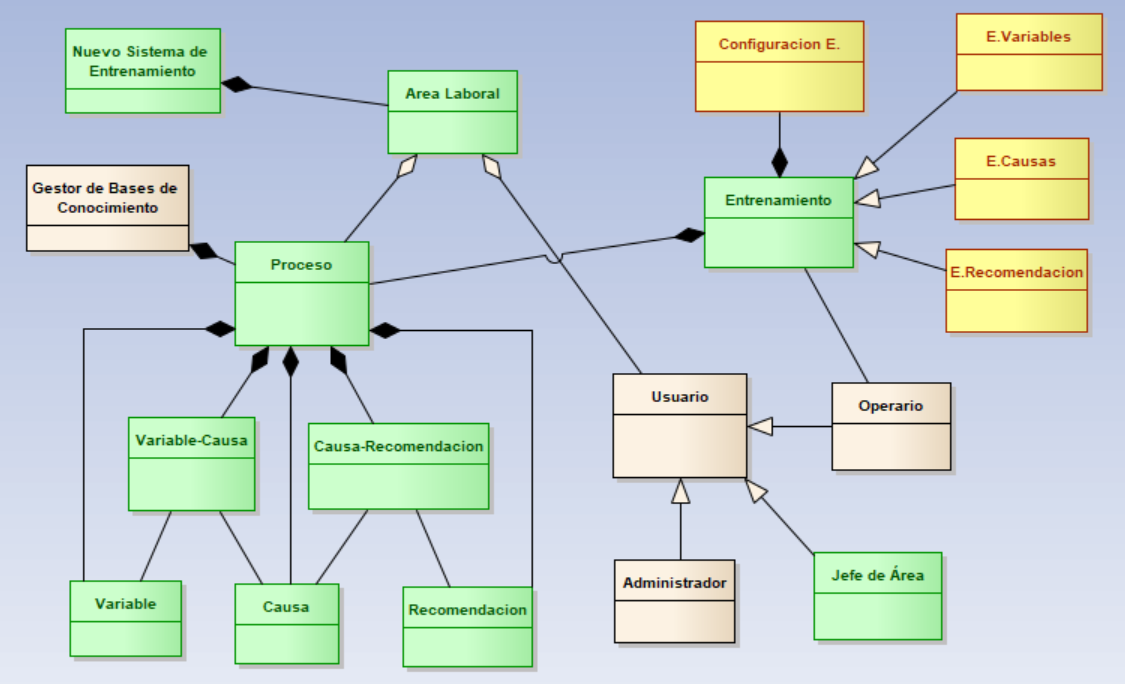
\includegraphics[width=0.65\linewidth]{imagen/dominio.png}
 \caption{Modelo de dominio}
 \label{fig:dominio} 
\end{figure}

Las entidades que contienen algunos cambios (\textsl{Tabla \ref{tab:ent-amarilla}}), indican que también se realizaron arreglos en las estructuras que estas seguían, es decir, variaciones en las clases del sistema.

\begin{table}[H]
\begin{center}
\begin{tabular}{ | c | p{5cm} |  p{5.7cm} | }
\hline
\textbf{Entidad} & \textbf{Descripción} & \textbf{Cambios}\\
\hline
Sistema SECPROIT & Representa el sistema & Cambian las clases que posee \\
\hline
Jefe de área & Es un tipo de usuario y administrar los procesos & Antes era especialista y solo creaba los procesos \\
\hline
Proceso & Representa los procesos & Se le agrega un nuevo atributo: configuración de entrenamiento \\
\hline
Entrenamiento & Representa el entrenamiento del usuario & Se le agrega nuevos intentos por cada etapa \\
\hline
\end{tabular}
\caption{Modelo de dominio: entidades que sufrieron cambios}
\label{tab:ent-amarilla}
\end{center}
\end{table}

La entidades que no fueron modificadas (\textsl{Tabla \ref{tab:ent-azul}}),  no sufrieron cambios porque, basadas en las tareas que desempeñan, no varían sus funciones en este nuevo modelo.

\begin{table}[H]
\begin{center}
\begin{tabular}{ | c | p{12cm} | }
\hline
\textbf{Entidad} & \textbf{Descripción} \\
\hline
Área & Representa el lugar donde laboran los trabajadores y es donde están presentes los procesos \\
\hline
Usuario & Representa a la persona que va interactuar con el sistema \\
\hline
Administrador & Es un tipo de usuario y se encarga de administrar las entidades del sistema (áreas y demás usuarios) \\
\hline
Operario & Es un tipo de usuario y se encarga de realizar los entrenamientos \\
\hline
Base de datos & Representa el archivo \textsf{anm} \\
\hline
Base de reglas & Representa el archivo \textsf{drl} \\
\hline
Drools & Es la entidad que permite ejecutar las reglas del proceso \\
\hline
Variable & Forma parte de la base de datos del proceso y contiene la información que se se evalúa en la primera etapa \\
\hline
Causa & Forma parte de la base de datos del proceso y contiene la información que se evalúa en la segunda etapa \\
\hline
Recm. & Forma parte de la base de datos del proceso, representa las recomendaciones y contiene la información que se evalúa en la tercera etapa \\
\hline
Variable-Causa & Forma parte de la base de reglas del proceso y contiene la información que se evalúa en la primera y segunda etapa \\
\hline
Causa-Recm. & Forma parte de la base de reglas del proceso y contiene la información que se evalúa en la tercera etapa \\
\hline
\end{tabular}
\caption{Modelo de dominio: entidades que no sufrieron cambios}
\label{tab:ent-azul}
\end{center}
\end{table}

Por último, las entidades nuevas (\textsl{Tabla \ref{tab:ent-verde}}) son clases que fueron incluidas con el fin de enmendar alguna limitación.

\begin{table}[H]
\begin{center}
\begin{tabular}{ | c | p{12cm} | }
\hline
\textbf{Entidad} & \textbf{Descripción} \\
\hline
Configuración & Es la configuración del entrenamiento de un proceso, es decir, un grupo de características determinadas en el entrenamiento \\
\hline
Etapas & Representa las etapas del entrenamiento \\
\hline
E-Variable & Es la primera etapa, donde se evalúan las variables \\
\hline
E-Causa & Es la segunda etapa, donde se evalúan las causas \\
\hline
E-Recm. & Es la tercera etapa, donde se evalúan las recomendaciones \\
\hline
\end{tabular}
\caption{Modelo de dominio: entidades nuevas}
\label{tab:ent-verde}
\end{center}
\end{table}

\subsection{Reglas del negocio}
Las reglas de un negocio son directrices y restricciones que ayudan a regular las operaciones de una entidad determinada. Para cada proceso existen reglas que deben seguirse durante la ejecución, ya que estas ayudan a definir \textbf{cómo} deben realizarse las tareas, por \textbf{quién}, \textbf{cuándo}, \textbf{dónde} y \textbf{por qué} \cite{Chisholm2007}. A modo de resumen, las reglas de un negocio son límites impuestos a las operaciones para que estén en sintonía con las políticas y objetivos de la institución.

En el sistema SECPROIT existen un conjunto de reglas primordiales que no se deben dejar de cumplir:
\begin{itemize}
\item Cada usuario debe poseer un único rol
\item Para poder introducir un nuevo usuario debe existir, al menos, un área laboral
\item Un usuario no puede pertenecer a más de un área
\item Solo puede existir un jefe de área por área
\item Para poder introducir un nuevo proceso debe existir, al menos, un área laboral
\item Un proceso no puede pertenecer a más de un área
\item Para generar un nuevo entrenamiento debe existir, al menos, un usuario que cumpla el rol de operario y un proceso que sea de la misma área
\item Para entrenar en la etapa de las causas debe haberse aprobado la etapa de las variables
\item Para entrenar en la etapa de las recomendaciones debe haberse aprobado la etapa de las causas
\item Los usuarios con rol de administrador son los únicos que pueden gestionar las áreas y las cuentas de los usuarios
\item No se puede eliminar la cuenta de un usuario
\item Los usuarios con rol de jefe de área son los únicos que pueden gestionar los procesos de sus áreas y configurar los entrenamientos
\item Los usuarios con rol de operario son los únicos que pueden entrenar
\item Para superar un entrenamiento se deben haber aprobado las tres etapas (variables, causas y recomendaciones)
\end{itemize}

\subsection{Diagrama de actividades}
El Lenguaje Unificado de Modelado (UML) incluye varios subconjuntos de modelos, entre los que se encuentran los diagramas de actividades. Estos diagramas son considerados diagramas de comportamiento, porque describen el comportamiento del sistema que representan \cite{Eriksson2000}.

En el diagrama de actividades del nuevo sistema de capacitación (\textsl{Figura \ref{fig:actividades}}) se pueden observar tres colores: azul, amarillo y verde. El color azul indica que el flujo funciona de la misma manera que en el SECPROIT, el color amarillo representa un ligero cambio y el verde, representa una acción totalmente nueva.

\begin{figure}[h]
\centering
 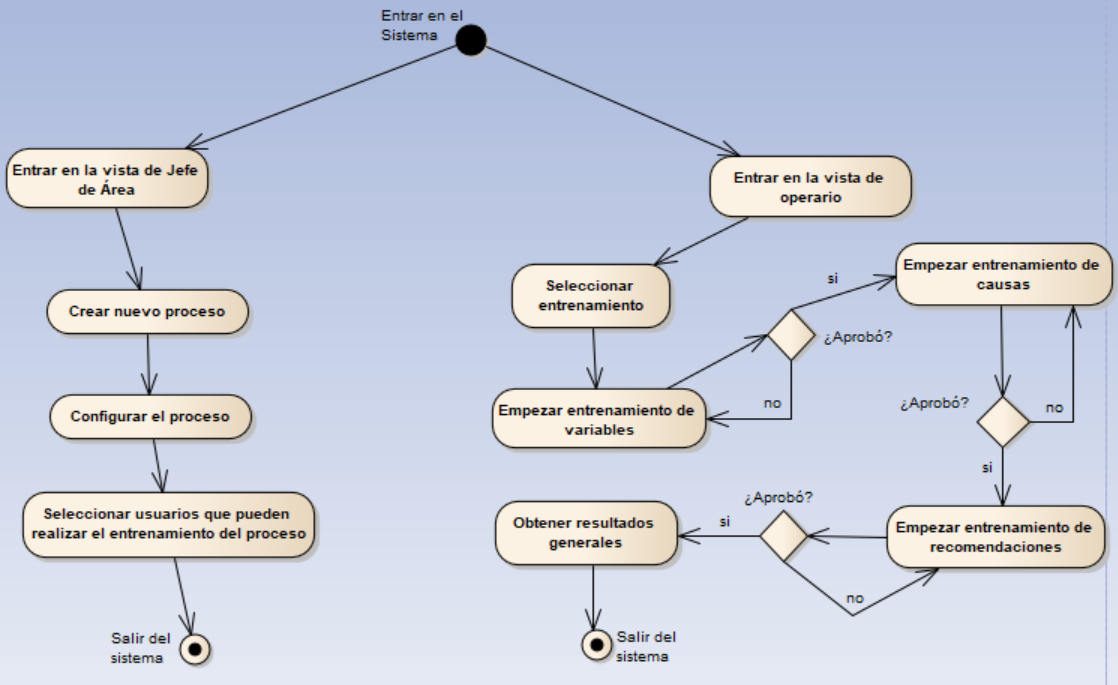
\includegraphics[width=0.65\linewidth]{imagen/actividades.png}
 \caption{Diagrama de actividades}
 \label{fig:actividades} 
\end{figure} 

\section{Captura de requisitos}
La extracción o captura de los requisitos en un sistema es una de las fases más críticas e importantes en el desarrollo de software. Esta fase tiene como objetivo descubrir y recoger todas las condiciones funcionales y no funcionales de una aplicación. La actividad de descubrimiento es una tarea más humana que técnica, ya que la mayor parte de las veces los usuarios no serán capaces de definir todas las condiciones \cite{Dave2022}. 

Para el desarrollo de este sistema se realizó un estudio de requisitos bastante extensivo. Se coordinó con los interesados y se acordó una lista de requerimientos funcionales y no funcionales.

\subsection{Requisitos funcionales}
Los requisitos funcionales son las declaraciones de los servicios que prestará el sistema. Cuando hablamos de entradas, no necesariamente hablamos sólo de los usuarios, pueden ser: interacciones con otros sistemas, respuestas automáticas, procesos predefinidos, entre otros. En algunos casos, los requisitos funcionales también establecen explícitamente lo que el sistema no debe hacer \cite{Dave2022}.

Entre los requisitos funcionales que debe poseer el nuevo sistema de capacitación, se deben incluir los cambios presentados en el modelo de dominio. Como resultado, los requisitos funcionales del nuevo sistema son:

\begin{itemize}
\item \textbf{Iniciar sesión en el sistema}: es una acción que todos los usuarios pueden realizar.
\item \textbf{Cambiar contraseña personal}: es una acción que todos los usuarios pueden realizar.
\item \textbf{Gestionar usuarios}: es una actividad desarrollada solo por los administradores. Se basa en introducir, modificar y desactivar o activar los usuarios del sistema, aunque también cuenta con una opción para restablecer la contraseña en caso de que el usuario la haya olvidado.
\item \textbf{Gestionar áreas}: es una actividad desarrollada solo por los administradores. Se basa en introducir, modificar y eliminar las áreas del sistema. Para poder eliminar un área laboral, esta debe estar vacía, es decir, que de ella no dependa ningún usuario.
\item \textbf{Ver acciones de los usuarios}: es una actividad desarrollada solo por los administradores. Permite observar, mediante una tabla, las acciones realizadas por los usuarios.
\item \textbf{Gestionar procesos}: es una actividad desarrollada solo por los jefes de área. Se basa en introducir, modificar y eliminar los procesos en un área laboral. Si se elimina un proceso, queda registro del mismo y los entrenamientos que se hayan realizado no se pierden.
\item \textbf{Configurar entrenamiento}: es una actividad desarrollada solo por los jefes de área. Consiste en asignar para cada proceso los estilos de pregunta que se pueden aplicar, la cantidad general de intentos, el tiempo máximo para realizar el entrenamiento y los usuarios que pueden evaluarse.
\item \textbf{Ver resultados de los operarios del área}: es una actividad desarrollada solo por los jefe de área. Permite observar, mediante una tabla, todos los resultados de los operarios que pertenezcan a su área.
\item \textbf{Entrenamiento}: es una acción desarrollada solo por los operarios. Consiste en evaluarse sobre un proceso productivo. Se deben responder un conjunto de preguntas por etapas para luego obtener un resultado general que será registrado en el sistema. Puede repetirse el entrenamiento de una etapa, tantas veces como el jefe de área decida.
\item \textbf{Ver resultados}: es una actividad desarrollada solo por los operarios. Permite observar, mediante una tabla, todos los resultados obtenidos en los entrenamientos realizados.
\end{itemize}

\subsection{Requisitos no funcionales}
Los requisitos no funcionales son condiciones que no se refieren directamente a las funciones específicas suministradas por un sistema (características de usuario), sino a las propiedades del mismo: rendimiento, seguridad, disponibilidad, entre otros. En palabras más sencillas, no hablan de lo que hace el sistema, sino de cómo lo hace. Alternativamente, definen restricciones del sistema tales como la capacidad de los dispositivos de entrada/salida y la representación de los datos utilizados en la interfaz del sistema \cite{Dave2022}.

En este caso, los requisitos no funcionales presentes en el nuevo sistema de capacitación son los mismos del SECPROIT:

\begin{itemize}
\item \textbf{Usabilidad}: se debe garantizar un ambiente de trabajo simple e intuitivo, ya que la mayoría de los usuarios no poseen experiencias con sistemas informáticos
\item \textbf{Seguridad}: la información del sistema solo puede ser manipulada por usuarios autorizados (aquellos que posean usuario y contraseña)
\item \textbf{Confiabilidad}: se deben evitar los enlaces rotos, los ficheros de los procesos deben ser validados antes de usarlos y se debe garantizar la confidencialidad de la información
\item \textbf{Disponibilidad}: la aplicación de mecanismos de seguridad no debe constituir un retraso para el uso del sistema, el software siempre debe estar disponible, así como brindar su información actualizada
\item \textbf{Software}: se debe tener instalado el JDK versión 1.8 y la aplicación PostgreSQL versión 9.1 (mínimo) para el manejo de la base de datos
\item \textbf{Hardware}: se necesitan 64MB de memoria RAM, un microprocesador Pentium II a 450 MHz (mínimo), un disco duro con capacidad libre de 4GB (mínimo) y un sistema operativo de entorno gráfico como Windows y Linux
\item \textbf{Portabilidad}: debe ser utilizado bajo sistemas operativos Windows o Linux, por lo que su desarrollo debe realizarse con un lenguaje y tecnologías capaces de brindar este soporte
\item \textbf{Restricciones en el diseño y la implementación}: debe desarrollarse sobre plataformas de software libre y código abierto y su lenguaje de programación debe ser Java, debido al uso de la herramienta \textsl{Drools}
\item \textbf{Políticos/Culturales}: debe encontrarse en idioma español
\end{itemize}

\section{Casos de uso}
Un caso de uso representa una unidad funcional coherente en un sistema, subsistema o clase. En ellos, uno o más actores interaccionan con las entidades que realizan las acciones. El modelado de estos casos de uso permite que los desarrolladores de un software y los clientes lleguen a un acuerdo sobre los requisitos y posibilidades que debe cumplir el sistema \cite{Kalaivani2004}.

\subsection{Diagrama de casos de uso}
Los diagramas de casos de uso muestran las relaciones entre las acciones de un sistema y sus actores. Estos modelos dan sólo una visión general y ayudan a interpretar y esclarecer los casos de uso \cite{Kalaivani2004}.

El diagrama de casos de uso del nuevo sistema de capacitación (\textsl{Figura \ref{fig:dcu}}) contiene tres colores diferentes: azul para los casos de uso que no han sido modificados, amarillo para los que sufrieron algún cambio significativo y verde para los casos de uso nuevos.

\begin{figure}[H]
\centering
 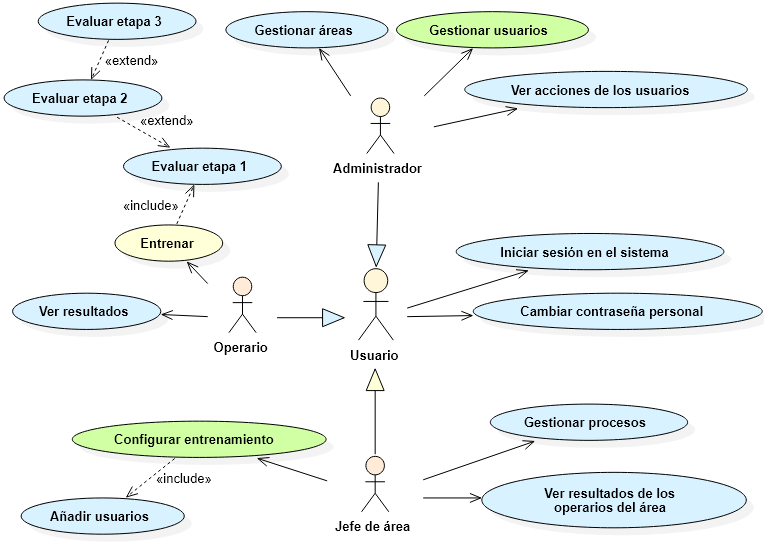
\includegraphics[width=0.65\linewidth]{imagen/dcu.png}
 \caption{Diagrama de casos de uso}
 \label{fig:dcu} 
\end{figure}

\subsection{Actores del sistema} 
Un actor puede referirse a cualquier entidad externa que interaccione con el sistema. No necesariamente coinciden con los usuarios. Un usuario puede interpretar distintos roles, correspondientes a distintos actores. Un actor puede desempeñar distintos papeles dependiendo del caso de uso en que participe \cite{Kalaivani2004}.

El Sistema Generador de Bases de Conocimiento (SGBC) es el encargado de confeccionar los ficheros de cada proceso dentro del sistema SECPROIT, como ya se explicó en el capítulo anterior. Sin embargo, este generador no se incluye como un actor, ya que no interactúa directamente con el sistema. Su relación es a partir de los ficheros que genera.

Los actores presentes en el nuevo sistema de capacitación (\textsl{Tabla \ref{tab:actores}}) están representados por tres roles: administrador, jefe de área u operario.

\begin{table}[H]
\begin{center}
\begin{tabular}{ | c | p{11cm} | }
\hline
\textbf{Actor} & \textbf{Descripción} \\
\hline
Usuario & Actor genérico que hace uso de las funcionalidades que son comunes \\
\hline
Operario & Actor que tiene acceso a los entrenamientos y posee un registro de sus resultados \\
\hline
Jefe de área & Actor que incluye los procesos a un área, decide cómo será el entrenamiento, qué usuarios podrán realizarlo y tiene acceso a los resultados de los operarios de su área \\
\hline
Administrador & Actor que gestiona las áreas, gestiona los usuarios y tiene acceso a un reporte de las acciones en el sistema \\
\hline
\end{tabular}
\caption{Actores del sistema}
\label{tab:actores}
\end{center}
\end{table}

\subsection{Especificación de los casos de uso}

\begin{table}[H]
\begin{center}
\begin{tabular}{ | c | p{3.5cm} |  p{7.5cm} |}
\hline
\textbf{Actor} & \textbf{Caso de uso} & \textbf{Descripción}\\
\hline
Administrador & Gestionar áreas & El actor puede introducir, modificar o eliminar las áreas del sistema \\
\cline{2-3}
& Gestionar usuarios & El actor puede introducir, modificar, dormir o activar a los usuarios del sistema \\
\cline{2-3}
& Ver acciones de los usuarios & El actor puede visualizar un registro con todas las acciones realizadas en el sistema \\
\hline
\end{tabular}
\caption{Casos de uso del administrador}
\end{center}
\end{table}

\begin{table}[H]
\begin{center}
\begin{tabular}{ | c | p{3.8cm} |  p{8cm} |}
\hline
\textbf{Actor} & \textbf{Caso de uso} & \textbf{Descripción}\\
\hline
Usuario & Iniciar sesión en el sistema & El actor debe introducir su nombre de usuario y su contraseña para iniciar sesión en el sistema \\
\cline{2-3}
& Cambiar contraseña personal  & El actor puede cambiar la contraseña que posee por defecto, por una de su preferencia \\
\hline
\end{tabular}
\caption{Casos de uso del usuario}
\end{center}
\end{table}

\begin{table}[H]
\begin{center}
\begin{tabular}{ | c | p{3cm} |  p{8.5cm} |}
\hline
\textbf{Actor} & \textbf{Caso de uso} & \textbf{Descripción}\\
\hline
Operario & Entrenar & El actor inicia el entrenamiento de un proceso \\
\cline{2-3}
& Entrenar en la primera etapa & El actor se evalúa en la primera etapa del entrenamiento (debe escoger las variables que se encuentran fuera de rango) \\
\cline{2-3}
& Entrenar en la segunda etapa & El actor se evalúa en la segunda etapa del entrenamiento (debe escoger las causas de las variables que se encuentran fuera de rango) \\
\cline{2-3}
& Entrenar en la tercera etapa & El actor se evalúa en la tercera etapa del entrenamiento (debe escoger las recomendaciones de las causas) \\
\cline{2-3}
& Ver resultados & El actor puede visualizar un registro con todos los resultados que ha obtenido \\
\hline
\end{tabular}
\caption{Casos de uso del operario}
\end{center}
\end{table}

\begin{table}[H]
\begin{center}
\begin{tabular}{ | c | p{3.5cm} |  p{7.5cm} |}
\hline
\textbf{Actor} & \textbf{Caso de uso} & \textbf{Descripción}\\
\hline
Jefe de área & Gestionar procesos & El actor puede introducir, modificar o eliminar los procesos de su área \\
\cline{2-3}
& Configurar entrenamiento & El actor decide para cada proceso cómo será el entrenamiento \\
\cline{2-3}
& Añadir usuarios & El actor decide para cada proceso los usuarios que lo pueden realizar \\
\cline{2-3}
& Ver resultados de los operarios del área & El actor puede visualizar un registro con todas las evaluaciones de los operarios de su área \\
\hline
\end{tabular}
\caption{Casos de uso del jefe de área}
\end{center}
\end{table}

\section{Modelo de datos}
Para el desarrollo de este sistema se utiliza, como gestor de base de datos, la herramienta PostgreSQL. En ella se almacena toda la información con la que se va a trabajar, incluyendo los ficheros \textsl{anm} y \textsl{drl} de los procesos. Por momentos determinados, esta información también se encuentra almacenada, de forma local y temporal, en clases del propio sistema, lo que permite un mejor manejo y control de los datos.

\subsection{Diagrama de Entidades y Relaciones (DER)}
Un Diagrama de Entidades y Relaciones (DER) es una herramienta que permite representar de manera simplificada los componentes que participan en un proceso, y el modo en el que estos se relacionan entre sí. Posee tres elementos principales: las entidades, los atributos y las relaciones \cite{Li2009}.

El diagrama de entidades de este nuevo sistema de capacitación (\textsl{Figura \ref{fig:der}}) contiene varias modificaciones con respecto al diagrama presente en el sistema SECPROIT. Para una mejor representación de los cambios, se tuvieron en cuenta una serie de colores:

\begin{itemize}
\item \textbf{Azul}: representa aquellas entidades que no sufrieron ningún cambio significativo con respecto al sistema SECPROIT
\item \textbf{Amarillo}: representa aquellas entidades que fueron modificadas, pero que siguen cumpliendo las mismas funciones
\item \textbf{Verde}: representa las entidades que son totalmente nuevas
\end{itemize}

\begin{figure}[h]
\centering
 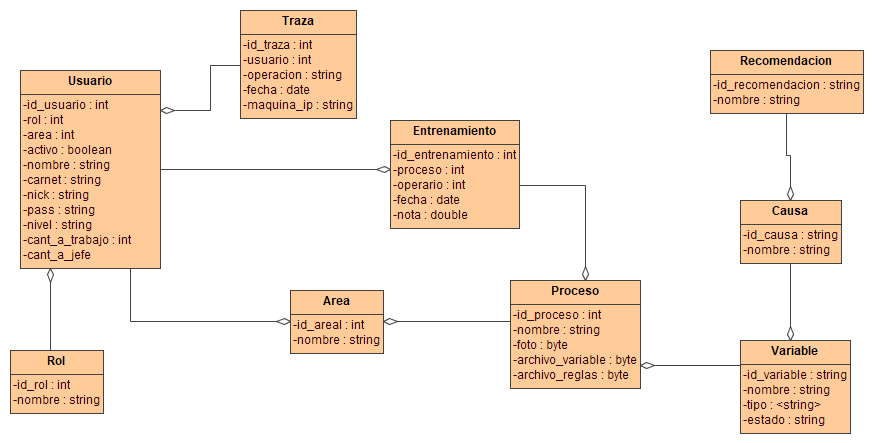
\includegraphics[width=0.65\linewidth]{imagen/der.png}
 \caption{Diagrama de Entidades y Relaciones (DER)}
 \label{fig:der} 
\end{figure}

En este diagrama no solo se cambiaron y se agregaron nuevas entidades, también se eliminaron algunas de las entidades presentes en el diagrama del sistema SECPROIT, debido a que ya no eran necesarias su funciones. Para realizar una comparación más detallada puede verse \cite{ElenaAcostaGil2018}, donde se encuentra el diagrama mencionado junto a su explicación. Las modificaciones realizadas (\textsl{Tabla \ref{tab:entidades}}) se hicieron con el fin de resolver algunas de las limitaciones presentes en el SECPROIT.

\begin{table}[H]
\centering
\begin{center}
\begin{tabular}{ | c | p{5cm} |  p{5cm} | }
\hline
\textbf{Entidad} & \textbf{Atributos}  & \textbf{Descripción}\\
\hline
Área & ID y nombre & No sufrió ningún cambio \\
\cline{1-2}
Traza & ID, usuario, acción y fecha &  \\
\cline{1-2}
Proceso & ID, nombre, foto, base de datos, base de reglas y área &  \\
\hline
Usuario & ID, nombre, carnet, sexo, nivel escolar, experiencia, años como jefe, usuario, contraseña, área, rol y activo & Se agregaron nuevos atributos que permiten conocer mejor al usuario\\
\hline
Configuración & ID, proceso, tiempo, cantidad de preguntas, cantidad de preguntas aprobadas y tipos de pregunta & Se agregó con el fin de poder configurar los entrenamientos \\
\hline
Entrenamiento & ID, operario, configuración de proceso, cantidad de intentos, cantidad de intentos aprobados, primera etapa, segunda etapa, tercera etapa y nota general & Se eliminaron los demás atributos que poseía \\
\hline
Etapa-Entrenamiento & ID, entrenamiento, tipo de etapa, tiempo, preguntas acertadas y nota & Se agregó para poder tener una pausa entre etapas y poder realizar más de una prueba por etapa \\
\hline
Variable & ID, nombre, tipo, valores y proceso & Se agregó en el sistema para agilizar el proceso de lectura \\
\cline{1-2}
Causa & ID y nombre &  \\
\cline{1-2}
Recomendación & ID y nombre & \\
\cline{1-2}
Variable-Causa & ID, variable y causa &  \\
\cline{1-2}
Causa-Recomendación & ID, causa y recomendación &  \\
\hline
\end{tabular}
\caption{Entidades del nuevo sistema de capacitación}
\label{tab:entidades}
\end{center}
\end{table}

\subsection{Diagrama de base de datos}
La herramienta utilizada para crear y gestionar la base de datos del nuevo sistema de capacitación (PostgreSQL), permite exportar un diagrama de la misma (\textsl{Figura \ref{fig:bd}}). En dicho diagrama se pueden apreciar las relaciones existentes entre las entidades del software y los atributos que poseen cada una.

\begin{figure}[H]
\centering
 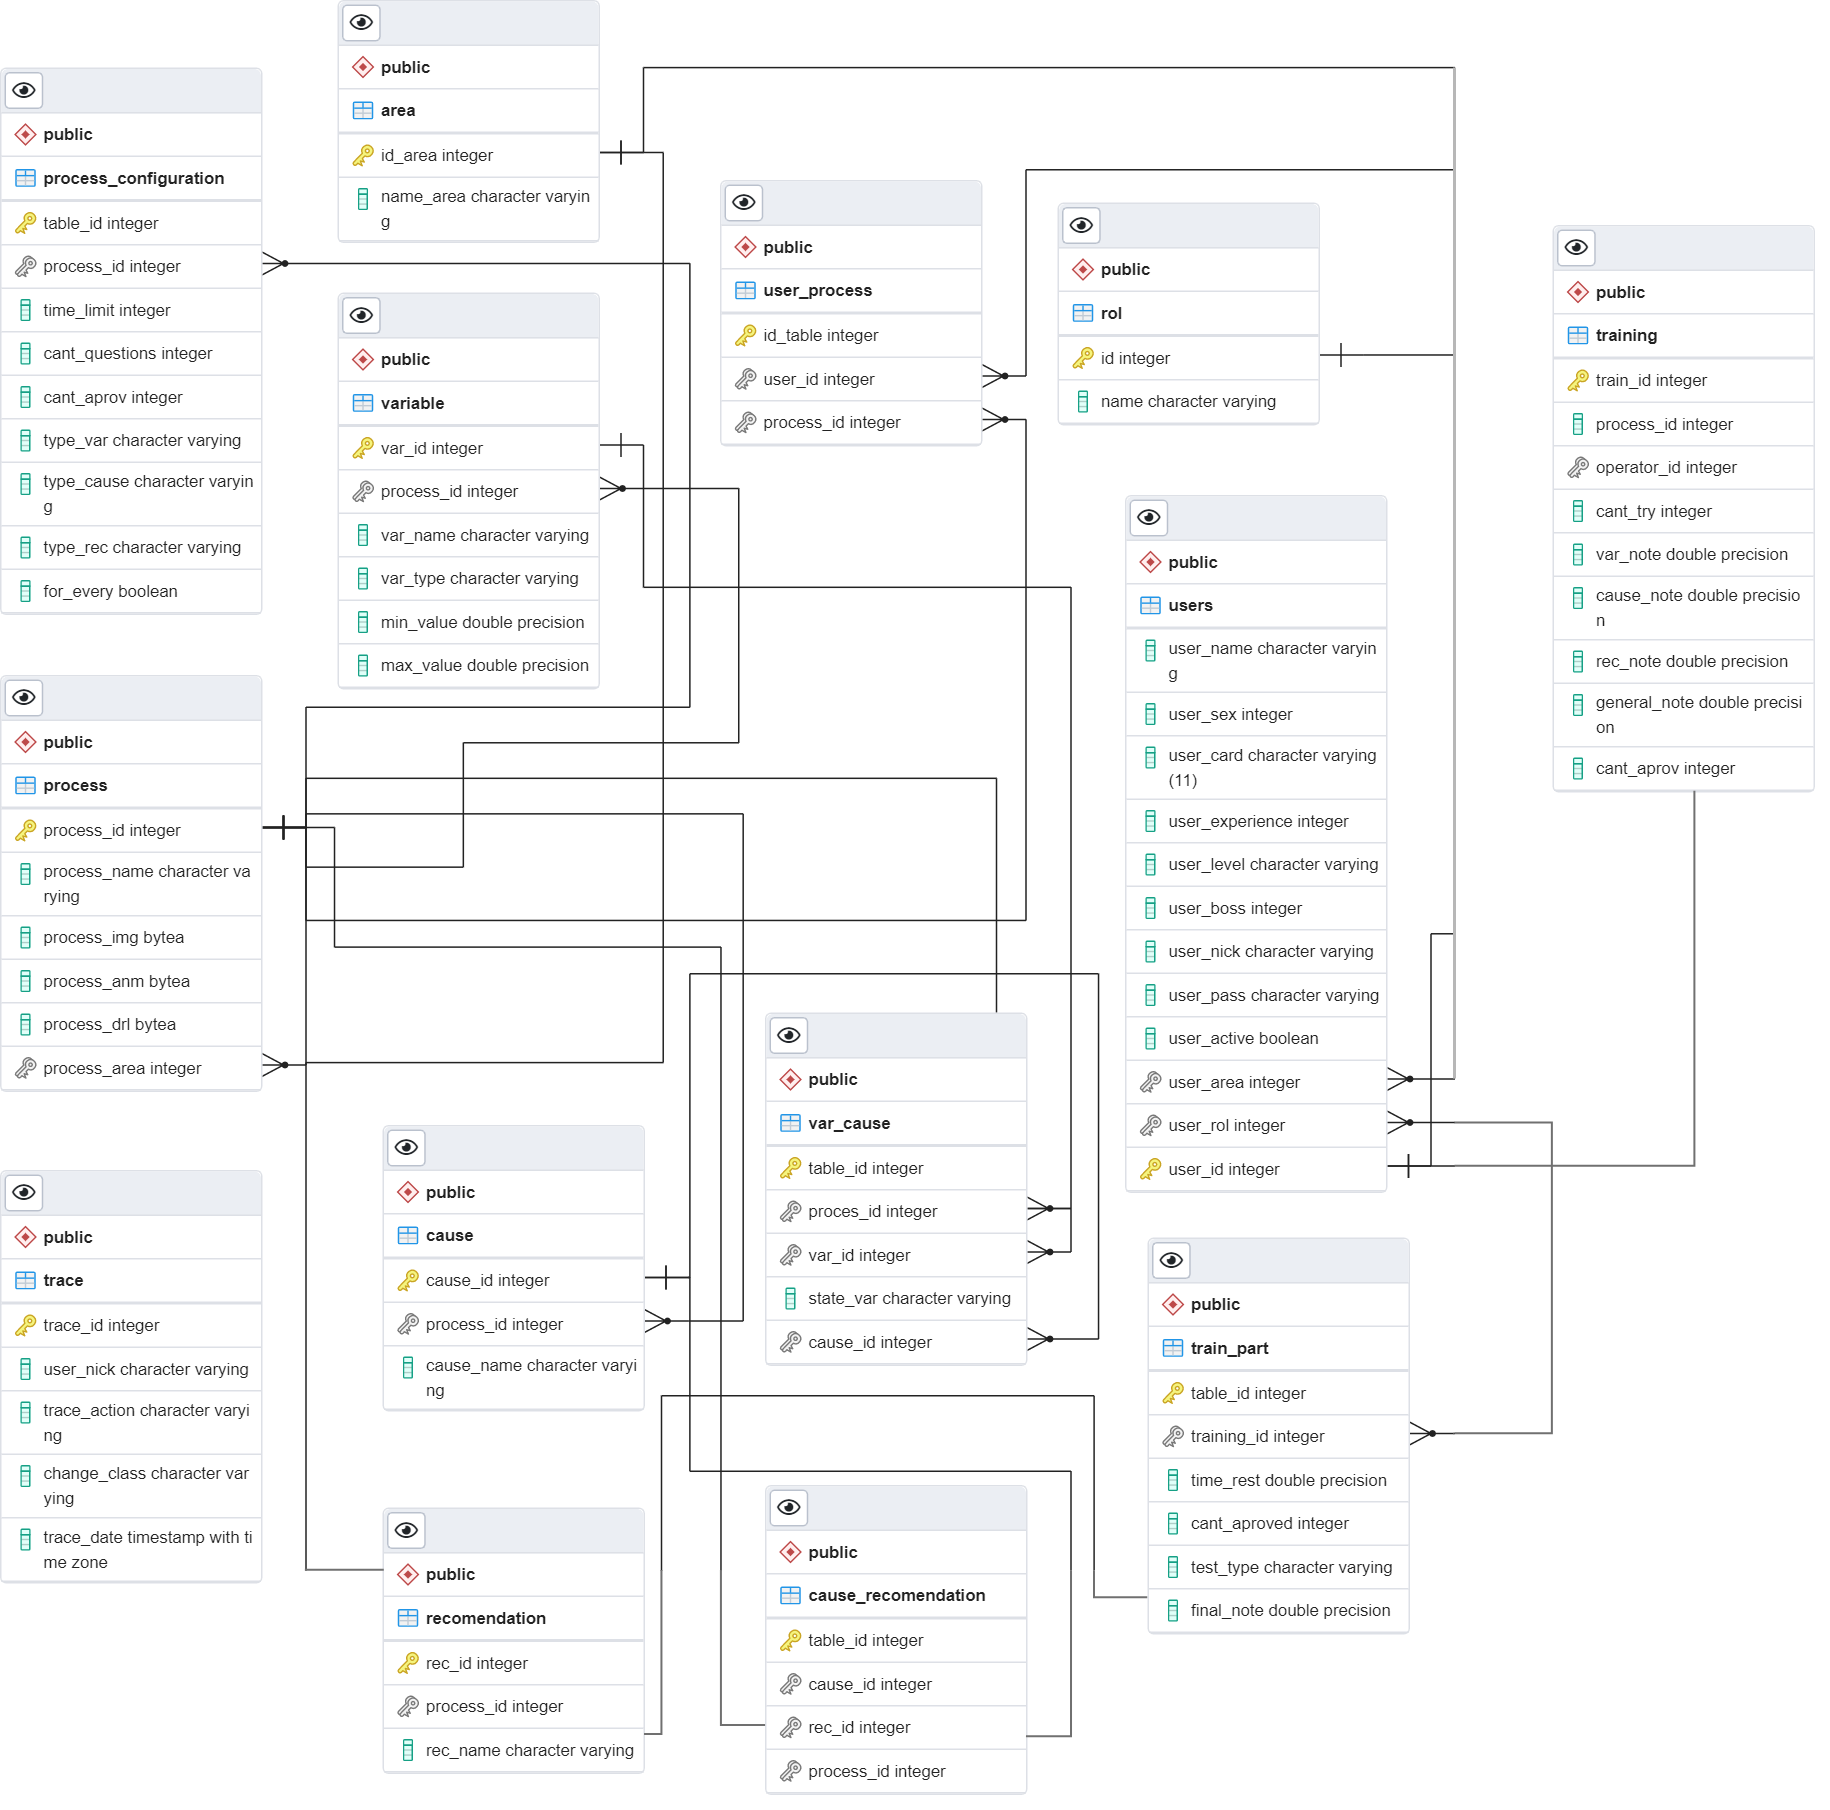
\includegraphics[width=0.9\linewidth]{imagen/bd.png}
 \caption{Diagrama de base de datos}
 \label{fig:bd} 
\end{figure}

\section{Arquitectura de paquetes del nuevo sistema de capacitación}
El patrón arquitectónico de capas ayuda a estructurar las aplicaciones, organizando las clases en grupos de subtareas, en donde que cada uno se encuentra a un nivel particular de abstracción. Se basa en una distribución jerárquica de los roles y las responsabilidades, para proporcionar una división efectiva de los problemas a resolver. Los roles indican el tipo y la forma de la interacción con otras capas y las responsabilidades, la funcionalidad que implementan \cite{Plecka2013}.

En este nuevo sistema de capacitación, se crearon un conjunto de paquetes  (\textsl{Tabla \ref{tab:paquetes}})  que agrupan las clases del sistema. Cada paquete responde a una funcionalidad o a una estructura específica, para ayudar con la organización del proyecto.

\begin{figure}[H]
\centering
 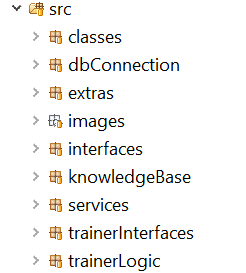
\includegraphics[width=0.27\linewidth]{imagen/paquetes.png}
 \caption{Arquitectura de los paquetes de clases}
 \label{fig:paquetes} 
\end{figure}

\begin{table}[H]
\centering
\begin{center}
\begin{tabular}{ | c | p{11.5cm} | }
\hline
\textbf{Paquete} & \textbf{Descripción}\\
\hline
classes & Contiene las clases que representan las entidades registradas en la base de datos \\
\hline
dbConnection & Contiene las clases que permiten establecer una conexión con la base de datos \\
\hline
extras & Contiene las clases que auxilian el proceso de generar las interfaces del sistema y clases que poseen funciones de validación \\
\hline
images & Contiene las imágenes utilizadas en el sistema \\
\hline
interfaces & Contiene las interfaces visuales del sistema \\
\hline
knowledgeBase & Contiene las clases que permiten establecer una conexión con el \textsl{JDrools}, así como las clases que auxilian el proceso de cargar y leer un fichero (todo lo relacionado con el sistema experto) \\
\hline
services & Contiene las clases que brindan un servicio a la base de datos (insertar, leer, modificar o eliminar) \\
\hline
trainerInterfaces & Contiene las interfaces visuales relacionadas con las etapas del entrenamiento \\
\hline
trainerLogic &  Contiene las clases que permiten el correcto funcionamiento de una etapa de entrenamiento \\
\hline
\end{tabular}
\caption{Descripción de los paquetes de clases}
\label{tab:paquetes}
\end{center}
\end{table}

\section{Proceso de entrenamiento}
Los entrenamientos están compuestos por tres etapas: variables, causas y recomendaciones. Cada etapa es decisiva en la evaluación final del entrenamiento, por lo tanto, se deben aprobar todas las etapas para afirmar que un entrenamiento fue completado. De lo contrario, el operario será notificado como suspenso en ese proceso.

Una de las funcionalidades presentes en el nuevo sistema de capacitación es la configuración de entrenamiento. Gracias a esta, un operario puede realizar varios intentos en una misma etapa, acumulando puntos positivos a su promedio, es decir, si suspende, tiene la oportunidad de volverlo a intentar. También se incluyeron nuevos tipos de preguntas, lo que aumenta el método de aprendizaje del adiestrado. 

Las preguntas de cada etapa se generan de forma aleatoria, incluyendo entrenamientos con todas las preguntas correctas o todas incorrectas. De esta manera se evita el fraude y el aprendizaje por memoria.

\subsection{Modelo matemático de la evaluación por etapas}
En el sistema SECPROIT, para evaluar una etapa se utiliza un método de evaluación por escala, es decir, dependiendo de la cantidad de preguntas acertadas se devuelve una evaluación de acuerdo a la escala que se tiene (muy mal, mal, regular, bien, muy bien y excelente). El sistema que utiliza para mostrar los resultados es el sistema de aprobado o no, dejando en claro el nivel de satisfacción según la escala mencionada anteriormente.

Este tipo de evaluación trae como resultado la desinformación del usuario, ya que no se puede apreciar a simple vista la evolución del mismo. Por esa razón, es necesario establecer un sistema numérico que permita observar el avance del operario.

En el nuevo sistema de capacitación se insertó un sistema de evaluación a base de fórmula, tomando en cuenta los parámetros de: tiempo y cantidad de preguntas correctas. El parámetro del tiempo, en este tipo de evaluación, es decisivo, porque el objetivo de este sistema es preparar a los operarios para situaciones reales y, en las industrias, mientras más rápido se resuelva una falla, menores problemas y daños ocasiona.

La fórmula utilizada en el nuevo sistema de capacitación es:

\vspace{0.2cm}
\begin{center}
\begin{Large}
\textbf{N} = (Ca/C + (Td/T \cdot  0.1))
\end{Large}
\end{center}
\vspace{0.15cm}

Donde \textbf{N} es la calificación obtenida en la etapa, \textbf{Ca} es la cantidad de preguntas acertadas, \textbf{C} es la cantidad de preguntas en total, \textbf{Td} es el tiempo demorado en responder todas las preguntas (en minutos) y \textbf{T} es el tiempo total (en minutos). Nótese que el tiempo es multiplicado por 0,1. Esto se debe a que el valor del tiempo es importante, pero no debe ser tomado como requisito fundamental, es decir, afecta la evaluación, pero no influye en el aprobado o desaprobado de la misma \cite{Castrillon2021}.

\subsection{Modelo matemático de la evaluación general}
En el sistema SECPROIT no existe la evaluación general de un entrenamiento. Por cada etapa se tiene una escala (muy mal, mal, regular, bien, muy bien y excelente) y a partir de esta se determina si el usuario aprobó o no.

En el nuevo sistema de capacitación se incorporó una fórmula para calcular la evaluación final de un entrenamiento a partir del promedio de las notas obtenidas por el usuario en cada una de las etapas. De esta manera se puede realizar un estudio más profundo y detallado de las habilidades de los operarios, así como extraer estadísticas generales con las notas de los usuarios.

La fórmula utilizada para obtener el resultado final del entrenamiento de un proceso es la siguiente:

\vspace{0.15cm}
\begin{center}
\begin{Large}
\textbf{Ng} = (E1 \cdot 0.4) + (E2 \cdot  0.3) + (E3 \cdot  0.3)
\end{Large}
\end{center}
\vspace{0.15cm}

Donde \textbf{Ng} es la calificación general del entrenamiento, \textbf{E1} es el promedio de las evaluaciones aprobadas de la etapa 1, \textbf{E2} es el promedio de las evaluaciones aprobadas de la etapa 2 y \textbf{E3} es el promedio de las evaluaciones aprobadas de la etapa 3. Nótese que el primer promedio se multiplica por 0,4 y los otros dos se multiplica por 0,3. Esto se debe a que el valor del resultado final es en base a 10 y a que la primera etapa (variables) es más extensa y más difícil que las otras dos etapas (causas y recomendaciones).

\section{Interfaces de usuario}
Algunas de las limitaciones presentes en el sistema SECPROIT se deben a sus interfaces de usuario:

\begin{itemize}
\item A pesar de ser una aplicación de escritorio, no presenta un icono de sistema que permita manejar su estado, es decir, no se puede minimizar ni encontrar con facilidad (Anexo \ref{fig:noIcono})
\item Contiene colores oscuros que generan poco contraste con las letras, lo que provoca un menor entendimiento y un mayor desagrado en los usuarios
\item En algunas de sus vistas los títulos aparecen cortados por los límites de la ventana (Anexo \ref{fig:titulo})
\item Algunas interfaces de usuario no presentan bordes, impidiendo que se puedan desplazar (Anexo \ref{fig:bordes})
\item Algunas ventanas necesitan ser ampliadas para poder visualizar todo su contenido, es decir, se muestra contenido a medias porque el tamaño de las visuales no es el adecuado (Anexo \ref{fig:tamano})
\item Las tres etapas del entrenamiento se muestran en la misma vista, si se suspende una, aparece espacio en blanco innecesario (Anexo \ref{fig:inn})
\end{itemize}

Con el desarrollo del nuevo sistema de capacitación se trataron de enmendar las limitaciones anteriores, quedando las interfaces de usuario de la siguiente manera:

\begin{itemize}
\item Se cambiaron los colores del sistema, predominando el color naranja gracias al estudio realizado en el capítulo 1 (Anexo \ref{fig:login}).
\item Se desarrolló una única vista central, en la que irán apareciendo las operaciones que el usuario desea realizar. Se organizó de esta manera para facilitarle al usuario las acciones y que no tenga que abrir y cerrar ventanas por cada operación (Anexo \ref{fig:principal}).
\item Se incluyó un icono de sistema, disponible en todo momento. Además, se habilitó la opción de agrandar o minimizar la ventana del software (Anexo \ref{fig:principal}).
\item Para la gestión de usuarios, se utiliza una tabla donde aparecen todos los usuarios del sistema, permitiendo un grupo de acciones a partir de su selección. Aplicando este método, se validan los enlaces rotos (Anexo \ref{fig:gestionUss}).
\item La configuración de un entrenamiento se realiza a partir de la acción de insertar o modificar un proceso. Los campos que se requieren completar se muestran con un valor por defecto para evitar errores de validación (Anexo \ref{fig:confEn}).
\item Para iniciar un entrenamiento se debe escoger, mediante una tabla, el proceso que se desea evaluar. Esto se hace para evitar enlaces rotos. Además, la tabla muestra el estado actual del entrenamiento de ese proceso: no iniciado, iniciado o terminado (Anexo \ref{fig:entrenamientos}).
\item Antes de iniciar el entrenamiento de una etapa, se le indica al usuario qué etapa va a realizar, cuántos intentos le quedan, cuántos necesita aprobar y las notas de las etapas anteriores (Anexo \ref{fig:eniniciado} y \ref{fig:einiciado}).
\item En el nuevo sistema de capacitación se incluyeron cuatro tipos de preguntas: verdadero o falso (Anexo \ref{fig:pregvar}), completar los espacios en blanco (Anexo \ref{fig:pregcaus}), selección múltiple y enlazar.
\item Los resultados del entrenamiento de una etapa se muestra a partir de una barra de progreso. Además, se le incluye la nota obtenida, la cantidad de preguntas aceptadas, la descripción de si aprobó o no y se señalan las preguntas falladas (Anexo \ref{fig:notas}).
\end{itemize}

\section{Conclusiones parciales}
Al concluir este capítulo se pueden arribar las siguientes conclusiones:
\begin{itemize}
\item El diseño de diagramas UML facilitó el proceso de desarrollo del nuevo sistema, porque brindó un vista precisa y detallada de lo que se quería obtener
\item El análisis y captura de requisitos permitió conocer las restricciones funcionales y no funcionales que debía seguir el sistema, y ayudó a decidir qué tecnologías usar en su desarrollo
\item Estructurar en paquetes las clases del nuevo sistema de capacitación permitió una mejor organización del mismo
\item Incluir un modelo matemático para la evaluación del entrenamiento permitió poder realizar nuevas estadísticas con las notas de los usuarios
\item El nuevo diseño de las interfaces de usuario brinda una mayor usabilidad al sistema en general
\end{itemize}

	%\chapter{Validación de la Solución Propuesta}\label{chap:3}
En el presente capítulo se presenta la validación de la herramienta desarrollada. Para ello se realizan un conjunto de pruebas funcionales, además se establece una comparación entre los resultados estadísticos obtenidos para diferentes juegos de datos. Dicho proceso parte de cómo la fase de análisis y diseño se unen para llevar a cabo el sistema propuesto.

\section{Pruebas Funcionales}
Las pruebas de software, o pruebas funcionales, son el proceso de ejecutar un sistema o componente para medir su calidad, con la intención de encontrar errores que aún no se descubren y el proceso orientado a demostrar que un programa realiza las funciones para las cuales fue construido.

El nivel de prueba que se utiliza es pruebas de sistema, donde se ejecutan en el sistema completo, buscando defectos tanto en aspectos generales como particulares del comportamiento del sistema, se prueban sus funcionalidades y las respuestas del sistema como un todo. Los tipos de pruebas que se realizan son funcionales, donde se prueba la ejecución correcta de las funcionalidades del sistema. El método que se utiliza es las pruebas de caja negra, que se llevan a cabo sobre la interfaz del software, los casos de prueba pretenden demostrar que las funciones son operativas, que la entrada se acepta de forma adecuada y que se produce un resultado correcto, así como que la integridad de la información externa. 

\subsection{Caso de Prueba: Gestionar Usuario}
\begin{figure}[h]
\centering
 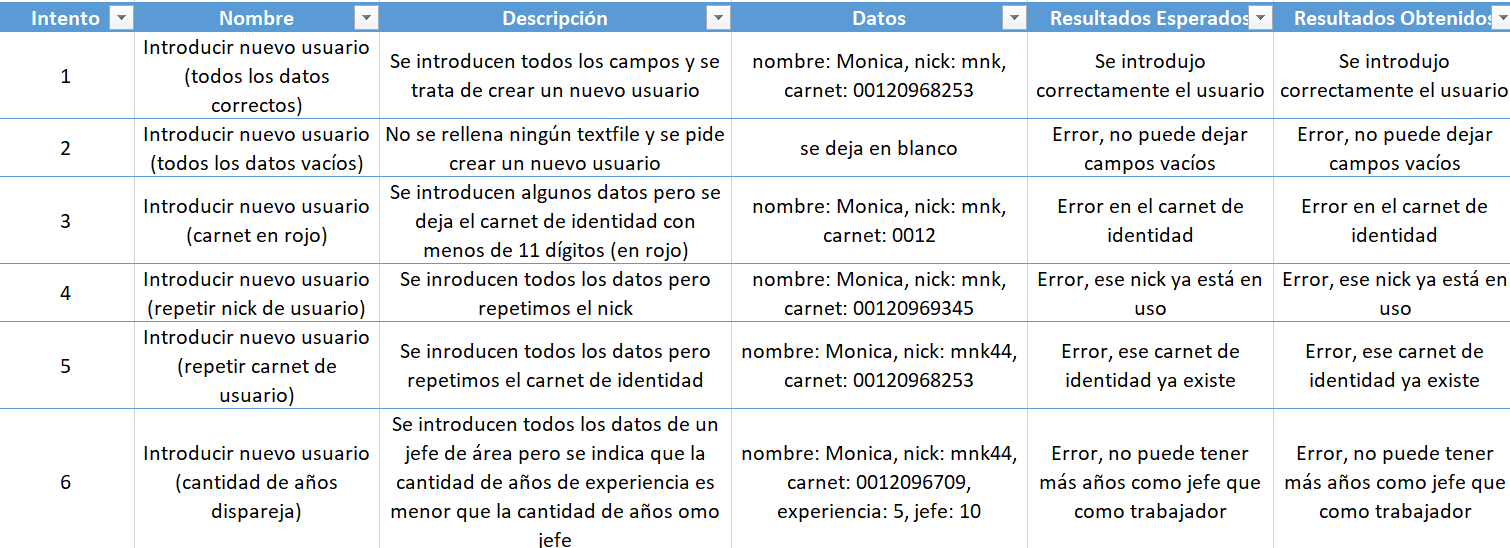
\includegraphics[width=0.8\linewidth]{imagen/introducirU.png}
 \caption{Caso de Prueba para Introducir Usuario.}
 \label{fig:introducirU} 
\end{figure}

\begin{figure}[h]
\centering
 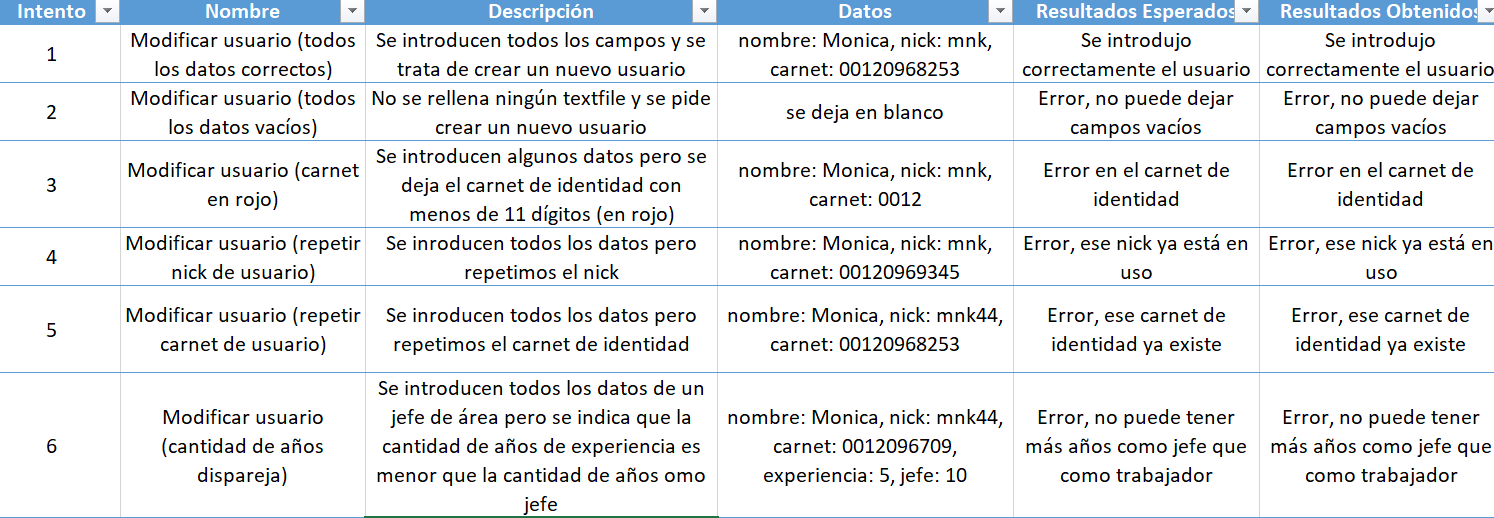
\includegraphics[width=0.8\linewidth]{imagen/modificarU.png}
 \caption{Caso de Prueba para Modificar Usuario.}
 \label{fig:modificarU} 
\end{figure}

En el caso de prueba de dormir a un usuario, la función recibe un identificador del usuario que debe dormir. No hay márgenes de error porque estos identificadores se obtienen a través de una tabla (Figura \ref{fig:img}), por lo que las pruebas con datos no fueron necesarias en este caso.

\subsection{Caso de Prueba: Gestionar Área}
\begin{figure}[h]
\centering
 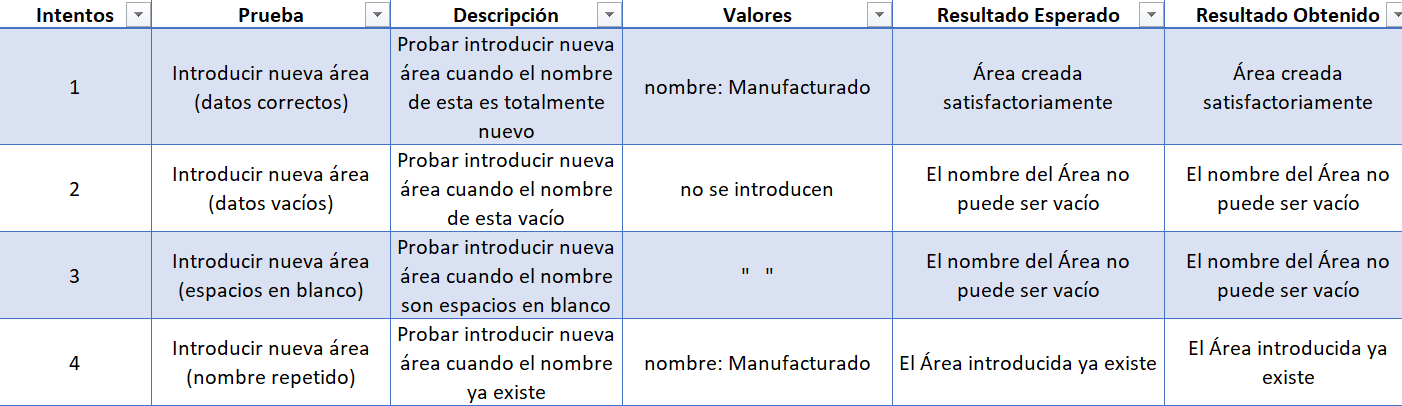
\includegraphics[width=0.8\linewidth]{imagen/introducirA.png}
 \caption{Caso de Prueba para Introducir Área.}
 \label{fig:introducirA} 
\end{figure}

\begin{figure}[h]
\centering
 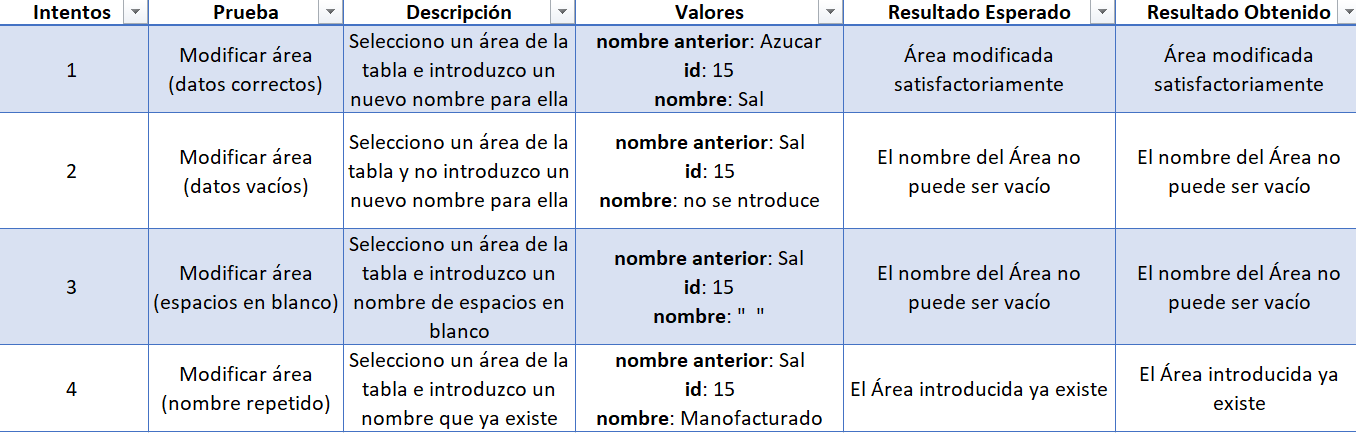
\includegraphics[width=0.8\linewidth]{imagen/modificarA.png}
 \caption{Caso de Prueba para Modificar Área.}
 \label{fig:modificarA} 
\end{figure}

\begin{figure}[h]
\centering
 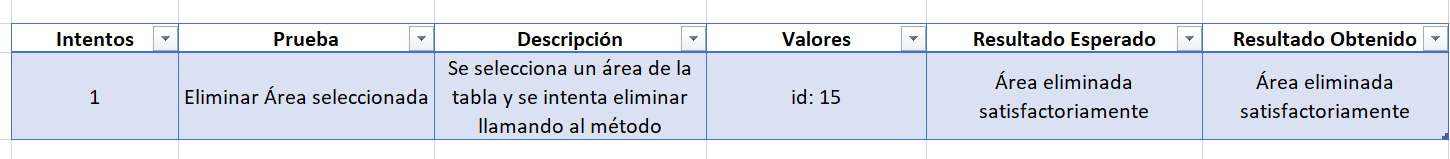
\includegraphics[width=0.8\linewidth]{imagen/eliminarA.png}
 \caption{Caso de Prueba para Eliminar Área.}
 \label{fig:eliminarA} 
\end{figure}

En el caso de prueba de eliminar un área, la función recibe un identificador del área que debe eliminar. No hay márgenes de error porque estos identificadores se obtienen a través de una tabla (Figura \ref{fig:img}), por lo que las pruebas con datos no fueron necesarias en este caso. Solo se activa el botón si el área puede ser eliminada.

\section{Análisis del Resultado de las Pruebas}
Con las pruebas realizadas se pudo comprobar el correcto funcionamiento del sistema, lo cuál resulta un logro para la investigación. También se pudo comprobar el correcto funcionamiento de las operaciones que eran necesarias modificar, tal como se propuso en un inicio.

\section{Conclusiones Parciales}
Durante este capítulo se realizaron numerosas pruebas al sistema para comprobar que los cambios realizados no afectaran sus funcionalidades. Como se pudo apreciar en los resultados obtenidos de las pruebas realizadas, los cambios no afectaron las funcionalidades, por lo que podemos afirmar que se cumplieron los objetivos de manera satisfactoria
	    
    \cleardoublepage
  \phantomsection
	\addcontentsline{toc}{chapter}{Conclusiones}
    
 % \chapter*{Conclusiones}
Al comenzar este trabajo se propuso una serie de objetivos específicos que ayudarían a completar el objetivo general del mismo. A lo largo, se ha ido completando cada uno de esos objetivos.
Tras cumplir satisfactoriamente con los objetivos específicos, se puede llegar a la conclusión de que se cumplió con el objetivo principal de la investigación. 

    
   \cleardoublepage
   \phantomsection
	\addcontentsline{toc}{chapter}{Recomendaciones}
	
	\chapter*{Recomendaciones}

	
	\cleardoublepage
	\phantomsection
	\addcontentsline{toc}{chapter}{Referencias bibliográficas}
	
	\nocite{*}
    \bibliographystyle{ieeetr}
	
	\bibliography{referencias/Referencias}
	\breakpage
	
	\phantomsection
	\addcontentsline{toc}{chapter}{Anexos}
	\pagestyle{fancy}
	
	\appendix
\clearpage{\renewcommand{\appendixname}{Anexo}
	
\end{document}